% Created 2018-07-18 Wed 13:26
\documentclass[12pt, letterpaper]{paper}
\usepackage[utf8]{inputenc}
\usepackage[T1]{fontenc}
\usepackage{fixltx2e}
\usepackage{graphicx}
\usepackage{longtable}
\usepackage{float}
\usepackage{wrapfig}
\usepackage{rotating}
\usepackage[normalem]{ulem}
\usepackage{amsmath}
\usepackage{textcomp}
\usepackage{marvosym}
\usepackage{wasysym}
\usepackage{amssymb}
\usepackage{hyperref}
\tolerance=1000
\usepackage{minted}
\usepackage{natbib}
\usepackage[margin=1in]{geometry}
\def\BigO{{\cal O}}
\renewcommand\maketitle{}
\DeclareMathOperator*{\argmin}{arg\,min}
\author{Timothy Schwieg}
\date{\today}
\title{Outline}
\hypersetup{
  pdfkeywords={},
  pdfsubject={},
  pdfcreator={Emacs 25.3.1 (Org mode 8.2.10)}}
\begin{document}

\maketitle
\bibliographystyle{chicago}

\begin{titlepage}
\centering
{\scshape\LARGE University of Central Florida\par}
\vspace{1cm}
{\scshape\Economics Department\par}
\vspace{1.5cm}
{\huge\bfseries A Structural Approach to Estimation of Valuations \par}
\vspace{2cm}
{\Large\itshape Timothy Schwieg\par}
\vfill
ECO 6936
\vfill

{\large \today\par}
\end{titlepage}


\section{Introduction}
\label{sec-1}
In this paper I seek to estimate the distribution of valuations as
well as the dynamics of the entry and distribution of the market of
cosmetic items in Counter-Strike: Global Offensive. Players may
receive certain items randomly as they play, and as they all have
private valuations, may wish to sell these items at market, or retain
them themselves. 

I seek to impose a strong structure on how these items are distributed
to players, and determine the nature of the valuations as well as how
many players are active in the market and how many enter or leave the
market over time. These primitives can then be extracted to determine
future policy decisions made about the implementation of newer items
into the game.

\section{Model}
\label{sec-2}

For any given item, assume that there is a mass of consumers who have
valuations based on some distribution $F_V$. With some exogenous
probability, some consumers are endowed with an item with probability
$\xi$. Consequently, the same distribution of valuations in those
endowed as well as those who are not endowed, even if there are
different numbers of people who are endowed. 

Because the process of granting items is random, it is in no way
efficient. No process exists that leads to the individuals who
value the good most receive it under the current function. In order to
achieve this efficiency, a market is implemented, taking the form
of a double auction.

It is known that double auctions  converge rapidly to a competitive
enviorment. The data pulled are relatively poor for extracting
valuations from the bids, as for much of the data the bids are not
observed; as a result attempting to identify valuations from the bids
would not work well. Even though the result is certainly possible for
double auctions under conditions such as sealed-bid, and one buyer and
seller, there has been no identification, based on a dominant or
equilibrium argument in the continuous double auction. 

Consequently, I shall abstract from the dynamics and the
mechanism of the double auction, and due to the large amount of
traffic, focus on its convergence into a competitive market. If the
market is efficient, then a matching between buyers and
sellers obtains after the trades where those with the highest
valuations have the items.

\subsection{The Matching Problem}
\label{sec-2-1}
Since it is known that the planner's problem of maximizing total
welfare, and the decentralized market are equivalent for this problem,
one can examine either interchangeably to provide motivation for the
problem.

The surplus generated by any exchange between a buyer and a seller is
given by the valuation of the buyer minus the valuation of the
seller. A central planner, who wishes to maximize the total surplus
then faces the question of finding a (partial) matching between buyers
and sellers such that the surplus generated is maximized. For some
arbitrary $I$ buyers and $J$ sellers:

\begin{align*}
\max_{\alpha_{i,j}} & \sum_{i=1}^I \sum_{j=1}^J \left ( V_i - V_j \right ) \alpha_{i,j }\\
\text{subject to: } & \forall j, 1 \leq j \le J \quad \sum_{i=1}^I \alpha_{i,j} \leq 1 \\
& \forall i, 1 \leq i \leq I \quad \sum_{j=1}^J \alpha_{i,j} \le 1 \\
\end{align*}

The constraints serve to require that each individual make at most one
exchange. One desirable result is that this linear program is always
maximized at integer values of $\alpha$. This ensures that the solution
contains no partial matchings.  Of interest as well is the dual of
the problem, which is specified below.

\begin{align*}
\min_{x,j} & \sum_{i=1}^I x_i + \sum_{j=1}^J y_j \\
\text{subject to: } & \forall i,j; \quad 1 \leq j \leq J, \quad 1 \le i \leq I\\
& x_i + y_j \geq V_i - V_j 
\end{align*}

The solution to this problem form the shadow prices of the exchange,
or the amount of surplus that a buyer or seller takes based on his or
her type. 

\subsubsection{Results}
\label{sec-2-1-1}
One important thing to note about the objective function is that it is
the buyer's valuation less the seller's valuation. This function
is both super-modular and sub-modular. This implies that for this
matching problem, both positive assortative mating and negative
assortative mating are supported. After some inspection, one can see
that even though the process will determine which of the sellers and
buyers match, any permutation of the matches is just as optimal.

That said, the dual of the problem does have a unique solution, as it is
the shadow price for the type of the seller and the buyer. These
values are the producer and consumer surplus for each type. Since it is
a competitive equilibrium, there is one price supported, as the good
is homogeneous, and the matching is occurring between valuations for the
good. The seller's valuation plus his shadow price will be equal to
the competitive price for all sellers who do exchange. 

For equal-sized buyer and seller valuations, this gives the intuitive
result that the lower half of the distribution of sellers will sell to
the upper half of the distribution of buyers, and we will have the
efficient result. As the size of the seller's mass shrinks, with the
rarity of the item increasing, a higher proportion of the sellers
choose to sell, and the receiving end of the distribution of buyers
shrinks, as the price increases. This is demonstrated below for
valuations that are distributed normally, with mean 35, and standard
deviation of 10. One Tenth of the population is endowed with the item.
The equilibrium price is calculated by taking the seller's valuation
plus his shadow price.

If one considers the decentralized market version of the problem, all
buyers are indifferent between the sellers they choose, as they must
give up the producer surplus to the seller, and as a result face a
constant price to buy from any seller type. 

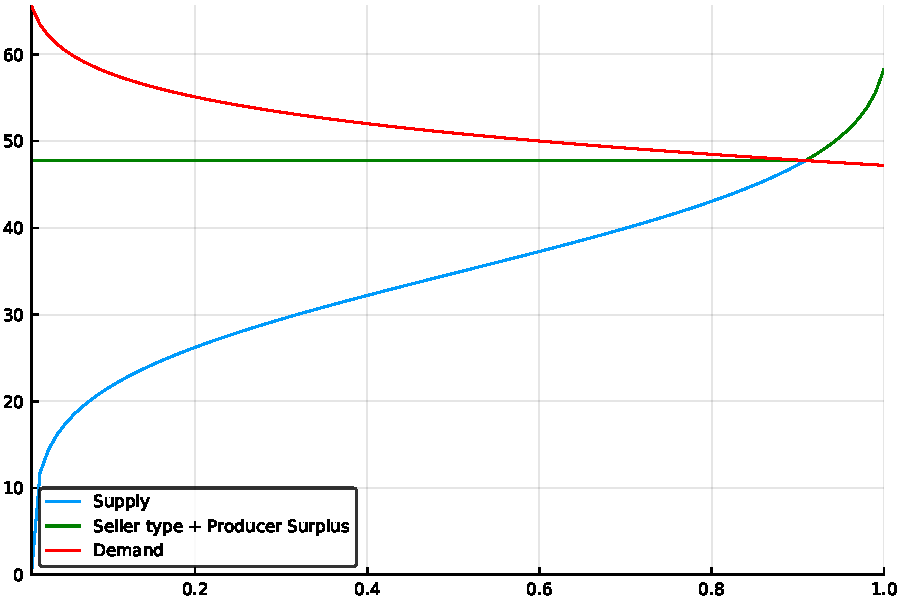
\includegraphics[width=.9\linewidth]{../Scripts/oneTenth.pdf}

The distribution of buyers has become truncated by the difference in
the number of buyers and sellers. To maintain the efficient outcome,
only the top $10$ percent of the buyers are able to purchase, and $90$
percent of the sellers are now selling. The result is a much higher
price.

While we would want to put down this change in the price to constant
demand, but a decrease in supply, the distribution of sellers has
remained constant, and in fact more of them are selling now. Within
the context of this matching model, the change in the relative sizes
of the population of suppliers acts to truncate the buyers rather than
lower the supply. It is important to note that these are not exactly
supply and demand in the normal sense, as instead of quantity, the
$x$-axis is the proportion of the sellers that exchange.

\subsubsection{Equilibrium}
\label{sec-2-1-2}
As a result of the lens in which this market is viewed, a slightly
different sort of equilibrium obtains. Although all the desirable
properties of an equilibrium hold, notably efficiency, and being in
the core, we are only examining exchanges in one good, so it remains a
partial equilibrium.

Assume that the valuations of the players are distributed
normally, as in the examples above. Then the supply function can be
written as $q = \xi \Phi \left ( \frac{ p - \mu }{\sigma} \right )$ and the demand
function can be written as: $q  = \left ( 1 - \xi \right ) \left [ 1 - \Phi \left ( \frac{
p - \mu }{ \sigma } \right ) \right ]$, $\xi$ is the percent of people endowed with
the item. In equilibrium, the quantity of buyers and sellers are
equal:

\begin{align*}
\Phi \left ( \frac{ p^* - \mu }{\sigma} \right ) &= \frac{1-\xi}{\xi} \left [ 1 - \Phi \left
( \frac{ p^* - \mu }{\sigma} \right ) \right ]\\
p^* &= \mu + \sigma \Phi^{-1} ( 1- \xi )\\
\end{align*}

Which tells us the price that the market supports is the average
valuation plus a component that depends on the rarity of the
item. Essentially this claims that the price is controlled by some
universal notion of value, such as the design of the skin, as well as
a rarity element that drives price up or down depending on how easy it
is to obtain.

\subsection{Identification}
\label{sec-2-2}
For some fixed $\xi$, this model gives a deterministic price for some
distribution of valuations. If one were to claim that the randomness
in this model arises from some unobserved error, then it remains
unidentified: $p^* = \mu + \sigma \Phi^{-1} \left ( 1 - \xi \right ) + U$. This model
depends on $\xi$ being exogenous. For many items, No published numbers of $\xi$
exist, and the mechanism for determining it is complicated at best.

\subsubsection{Estimating $\xi$}
\label{sec-2-2-1}

If one were able to estimate $\xi$, then the problem becomes one of
regression, and the covariates suffer from measurement error. This
would lead to biased and inconsistent estimates of the
coefficients. Clever rearrangement of the model might allow for
estimation, it is quite difficult to estimate $\xi$ outside of the
model. Crude estimates of $\xi$ may be able to be obtained using the
number of creates sold and the probabilities of each item being
unboxed by the item. However there are several complications that make
this almost impossible to handle.

\begin{itemize}
\item No data concerning the actual inventories of active
players exists. Players are able to set their inventories as private,
preventing anyone from seeing their contents.
\item Items can be combined into other items of higher quality, and there
is no data on the percentage of times this has been done.
\item The actual drop rate of the items is unknown, and the amount of
possible drops is limited to a only two per week per player. There
are no reliable estimates of the drop rate, nor what factors affect
it.
\end{itemize}

Since rare items are obtained almost exclusively through opening loot
boxes, one could obtain an estimate of the percentage of people
endowed with the item by taking the number of the lotteries sold and
multiplying it by the probability of obtaining that particular item in
the lottery. However the error cannot be quantified, and any
regression coefficients remain biased and inconsistent.

\subsubsection{Using the Quantity sold to approximate}
\label{sec-2-2-2}

All of the calculations so far have only used the price data, but one
may be able to use the quantity sold for a useful calculation. Since
the amount that is sold is determined solely by the percentage of the
population that receives the item, and the distribution is important
only for calculating the price that the item costs, one may use the
quantity of an item sold divided by the number of active players to
determine the percentage of the population that has
exchanged. Although this cannot account for exchanges that did not
take place on the market, it is still the best estimate that can
likely be gathered from the data.

For each item sold, there are different qualities
sold at market, and the probability of obtaining each quality is
known, one may form the estimate for each of the different
qualities. This allows us several values of $\xi$ observed, for which we
will have to assume that the mean is constant. However, this forces a
zero restriction of quality on the mean of the valuations, which is a
rather unreasonable assumption. By approaching the model this way, it
claims that the differences in prices between the different qualities
of items is driven solely by the probability of them being
dropped. This is unreasonable. Any attempt to put indicators for the
quality inside the mean will cause there to be colinearity in the
covariates, and linear regression will not produce a result. 
If however, we are willing to accept this mispecification error as
small enough to not cause problems, or if we only examine the highest
qualities among which there is almost no discernible difference, we
can estimate this model using linear regression. 

Since only the drop rate will be measured will be measured with error,
we need only rearrange the regression so that the drop rate is the
dependent variable, for which measurement error does not induce bias
and inconsistency. The estimable model would then be:

\begin{align*}
\Phi^{-1} ( 1- \xi ) = \frac{p^*}{\sigma} - \frac{\mu}{\sigma} \\
\Phi^{-1} ( 1- \xi ) = \beta_0 + \beta_1 p^* \\
\end{align*}

This method can be estimated using linear regression, and the values
of $\beta$ can be adjusted to determine the true values of the $\mu$ and $\sigma$ for
the distribution. All these results are driven by forcing the
quality to have no effect on the mean, and the magnitude of this error
cannot be observed. What we would like to seek is another way to
observe changes in $\xi$ that does not require such a strong assumption.

\subsection{Dynamic Approach}
\label{sec-2-3}
One possible way to handle the identification is to use the only
covariate that has a zero restriction on the mean: time. Consider a
series of time intervals, in which there is a matching device. In each
interval, a percentage of the population is awarded the item, and the
matching device functions as above. We may use the same strategy as
above, estimating $\xi$ using the quantity sold over the total number of
players in the time interval, and this in fact may be more precise
than the estimate used above. However this number can change over
intervals, giving us the changes in $\xi$ needed to identify the mean and
the standard deviation in our model.

First consider the model with no entrants. After the initial
exchange, those that do not have the item are random attributed the
item again, but their distribution is no longer the initial
distribution, it has been conditioned on losing the top portion of its
mass. Therefore the distribution of those that are possible sellers is
a mixture of this truncated distribution, and the top portion that
left the potential buyers. In this model, the top portion of
those that have the item will never sell it, as the valuations of
those that do not are all strictly below them: consider the
seller distribution to be a percentage of the buyers. The process then
repeats, albeit with a slightly truncated portion of the valuation
function. 

This model also more captures more elements of the market than the
original, as it can explain the behavior observed of a high initial
price, and it slowly dropping to some equilibrium level. With an
explanation of the dynamics of the process in place, we can look at
the entire lifetime of the item, and we only have to control for the
truncation of the valuations for the demand. 

As long as there is no entrance of individuals into the model, the
price will necessarily decrease. One useful result of doing this is
that we may be able to get a more precise estimate of the drop rate,
by looking at the number sold in the first interval that the item was
on the market, as it is far less influenced by exchange and other
unobserved factors. This number divided by the total number of active
players will likely give a much better estimate of the proportion of
players who receive the item per interval.

\subsubsection{Specification}
\label{sec-2-3-1}

Let us be specific with the notation used in this model. For each time
period $t$, the drop rate to individuals estimated is given by: $\xi$$_{\text{t}}$. The
price observed in that period is $p_t$. In the first time period,
everything proceeds according to the previous model. However in the
second time period, allow the top $\xi$$_{\text{0}}$ percent to exit the
model. There are $N(1-\xi_0)$ people remaining, of which $\xi$$_{\text{1}}$ have received
the item, so the mass of suppliers is: $\xi_1 (1-\xi_0)N$. The mass of the
buyers is: $(1-\xi_1)(1-\xi_0)N$. 

\begin{align*}
\Pr \left [ V_1 < v | V_1 < F_V^{-1}( 1 - \xi_0 )^{} \right ] &=
\frac { F_V ( v ) }{  F_V ( F_V^{-1} ( 1 - \xi_0 ) ) } = \frac{ F_V (v)
}{1 - \xi_0}\\
q_s &= N ( 1-\xi_0 )\xi_1 \left [ \frac{\Phi \left ( \frac{ p - \mu }{\sigma} \right )}{ 1 - \xi_0 } \right ]\\
q_d &= N ( 1-\xi_0 )(1-\xi_1) \left [ 1 - \frac{ \Phi \left ( \frac{
p - \mu }{ \sigma } \right ) }{ 1 - \xi_0 } \right ]
\end{align*}

We can continue the process, noting that with each truncation, there
is a multiplication of $(1-\xi_t)$ in the denominator of the supply
function.

\begin{align*}
q_s &= N \prod_{t=1}^{T-1} (1-\xi_t ) \xi_T \frac{\Phi \left ( \frac{ p - \mu }{\sigma} \right )}{ \prod_{t=1}^{T-1} ( 1 - \xi_t ) }\\
q_d &= N \prod_{t=1}^{T} ( 1- \xi_t ) \left [ 1 - \frac{ \Phi \left ( \frac{
p - \mu }{ \sigma } \right ) }{ \prod_{t=1}^{T-1} (1 - \xi_t ) } \right ]\\
p_T^* &= \mu + \sigma \Phi^{-1} \left [ \prod_{t=1}^T ( 1 - \xi_t ) \right ]\\
q_T^* &= N \xi_T \prod_{t=1}^T ( 1 - \xi_t )\\
\end{align*}

\subsection{Estimation}
\label{sec-2-4}
It is known that in each time period, the distribution of supply and
demand is binomial. However the difference between two binomial
distributions that are not independent is difficult to estimate using
likelihood methods. As a result, the generalized method of moments
will be utilized. Since the price is uniquely defined in each time
period, as is the quantity supplied, the question of estimation is
feasible.

In each time period T, there exists two moment conditions specified,
one for price, and one for quantity. Under the specification for the
model, for each time period T: $F_V ( p_T^* ) = \prod_{t=1}^T ( 1 - \xi_t )$ and
$q_T^* = \xi_T \prod_{t=1}^T ( 1 - \xi_t )$. This provides us with 2T moment
restrictions on the model, and allows for estimation of up to 2T
parameters. 

A distinction must be made between observations and time
periods. The data are divided into the median price and quantity
sold in each day, and the question of how many data points are in a
time period exists. For the purposes of the estimation in this paper,
I will use 5 observations per time period. If there are N
observations, then there are $T = \ceil{ \frac{ N }{5} }$ time periods.

For the model specified with T time periods, and for a distribution of
prices of log-normal, there are 2 parameters for the distribution, and
T parameters for the $\xi$. There are 2T moment restrictions, so the model
is in fact over-identified. This allows us to test the specification
for our model using the Sargan-Hansen J-test.

\subsubsection{Complications}
\label{sec-2-4-1}

One important complication is that there exists a price-floor in the
market. No item is able to be sold at less than \$ 0.03, this means
that for all data points where the price is at this floor, the
equilibrium condition is not binding. Since a price floor leads to
excess supply at the binding price, the only condition that remains
binding is that quantity demanded at the given price is equal to the
quantity sold. Denote K as the number of time periods in which the
price floor is binding.

This condition is written as: $q_d^T = N \prod_{t=1}^T \left [ 1 - \frac{ F_V (
p_T^* ) }{ \prod_{t=1}^{T-1} ( 1 - \xi_t ) } \right ]$. For each time period where
the price is at the floor, there is only one moment condition. For
this model, this implies that there must be at least two time periods
where the price is above the floor in order to identify the
model. This condition is upheld in all the data sets examined in this
paper, and effectively reduces the number of moments. In more
complicated settings with more primitives in the model, this could
become an important problem, as the current specification has the
equilibrium price converging to zero in time.

\subsubsection{Implementation}
\label{sec-2-4-2}
Consider a function g(Y$_{\text{t}}$ ,$\mu$,$\sigma$,$\xi$) which gives the moment condition for
each time period, evaluated at the t$^{\text{th}}$ element in that time
period. Under the Null Hypothesis that this model fits the data, then
the expected value of this function is zero.
\begin{equation*}
\mathbb{E}[ g( Y_t, \mu, \sigma, \xi ) ] = 0
\end{equation*}

We seek to estimate the parameters $\mu$, $\sigma$, $\xi$ by minimizing the sample
analog of this with respect to a weighting matrix W. The sample analog
is formed by averaging the data found contained in each time period.
$\hat{m} ( \mu, \sigma, \xi ) = \frac{ 1 }{ M } \sum_{m=1}^M g( Y_m, \mu, \sigma, \xi )$. Let us
combine the parameters of the model into a vector $\theta$. Our goal then
becomes to estimate a value of $\hat{\theta}$ by minimizing the quadratic
form of $\hat(m)$ with respect to matrix W.

\begin{equation*}
\hat{\theta} = \argmin_{\theta} \hat{m}( \theta )' W \hat{m}( \theta )
\end{equation*}

The choice of W is selected by first choosing a positive definite
matrix W, and estimating the model, and then estimating the matrix by
the following method:

\begin{align*}
\hat{W_i} &= \left [ \frac{1}{M} \sum_{m=1}^M g(Y_m, \hat{\theta_{i-1}} ) g( Y_m, \hat{\theta_{i-1}} )' \right ]^{-1} \\
\hat{\theta_i} &= \argmin_{\theta} \hat{m}( \theta_i )' \hat{W_i} \hat{m}( \theta_i ) \\
\end{align*}

This process is then continued until the value of $\theta_{i-1}$ is a
minimizer for W$_{\text{i}}$. This iterated GMM estimator is invariant to the
scale of the data, which is important in this model, as the price and
the quantity data are of wildly different magnitudes. (Cite
Hamilton 1994) This method is also asymptotically equivalent to the
Continuous Updating Efficient GMM, but does not have as many numerical
instabilities.  This process is complicated by $\hat{W_i}$ being of
rank $\min\{ M, 2T - K \}$. If the matrix is not of full rank, then it
is not invertible, and we cannot estimate the model. In order to
ensure that it has full rank, we add a positive number times the
identity matrix to ensure that $\hat{W_i}$ is both positive definite
and invertible.

The Model was estimated using the code found in the file
\texttt{dataTest2.jl} using the programming language Julia. Utilizing the
package \texttt{Optim.jl}, the objective function was minimized using the
BFGS algorithm. This ensured that numerical problems that could arise
out of calculations of inverting a small hessian were avoided. Several
of the fits are shown below.

\subsubsection{Testing}
\label{sec-2-4-3}

Since our model is over-identified, we are able to test for model-fit
using the J-test for model fit. Formally, we are testing the
hypothesis that $M \hat{m} ( \hat{\theta} )' \hat{W} \hat{m} ( \hat{\theta}
) = 0$. Since there are 2T - K moments in the
model, and T + 3 primitives in the model, the J-statistic is
distributed $\chi$$_{\text{T-K-3}}^{\text{2}}$. For several of the cases examined, a table
breaking down the model fit is shown.

\begin{center}
\begin{tabular}{lr}
Case & Sargan Test p-Value\\
Glove Case & 1.0\\
Huntsman Case & 0\\
Chroma Case & .89\\
\end{tabular}
\end{center}


Of interest is the question of whether or not there has been a
constant drop rate of an item to users in the game over time. This can
be written in the form of: $\textbf{\xi} = \textbf{1} \xi$. That is,
\textbf{\xi} is constant over the entire lifetime of the model. This
hypothesis can be tested with a Likelihood-Ratio test. We estimate the
model under the null and the alternate, and the difference in the
J-stastic is distributed $\chi$$_{\text{T-1}}^{\text{2}}$. 

\begin{center}
\begin{tabular}{lr}
Case & LR Test p-Value\\
Glove Case & 1.0\\
Huntsman Case & 0\\
Chroma Case & .89\\
\end{tabular}
\end{center}


\subsection{Market Entry}
\label{sec-2-5}

While the distribution model does describe several of the price
processes quite well, it struggles to rationalize the nearly constant
quantity of items sold in each period. One way to explain that is to
allow for market entry over time.

Consider the case in which the number of entrants in the market is not
held constant, but new entrants to the market have the same
distribution function as older ones. As a result, the distribution of
the buyers in the following period is now a mixture
distribution. Since we could now find a buyer of the highest
valuation, it is possible that sellers who had previously bought might
be willing to sell again. As a result, the entire seller's
distribution must be considered as well, as a mixture of the highest
portions of demand, and the currently endowed in that instance. 

Consider the model where, after the first exchange of items, $\lambda$$_{\text{0}}$
percent of N people enter the market, drawing their valuations from a
potentially different distribution. Then the endowment process is
repeated, and exchange occurs. After this process, $\lambda$$_{\text{1}}$ percent of the
N(1+$\lambda$$_{\text{0}}$) people enter the market. That is, $\lambda$$_{\text{t}}$ is the proportion of the
inhabitants of the market that enter the market in time period
t. However, they enter the market after the exchange has
occurred. This ensures that there is no entrance in the first time
period.

The distribution of buyers and sellers remains binomial. However,
since all sellers are possible sellers now, the distribution and mass
of the buyers and sellers has become noticeably more complex. the mass for the seller's
distribution is noticeably more complex. The mass of the sellers is
now the sum of the mass of the buyers times the percent of people
endowed in each time interval. That is, in time period one, the
sellers received $N \xi_0$ mass, and the mass of the buyers was:
$N(1-\xi_0)$. However, then $N\lambda_0$ people arrived, and for time period one
the buyers had mass: $N( 1 -\xi_0 + \lambda_0)(1-\xi_1)$, and the sellers had mass:
$N \xi_0 + N(1-\xi_0 + \lambda_0)\xi_1$. 

The mass of the buyers and the sellers continues on this trend and is
given by:

\begin{align*}
M_B(T) &= ( 1 - \xi_T ) \left [ M_B(T-1) + \lambda_{T-1} \prod_{t=1}^{T-2}( 1 + \lambda_t )N \right ] \\
M_S(T) &= N \sum_{i = 0}^T \xi_i \prod_{t=1}^{i-1} ( 1- \xi_t + \lambda_t )\\
\end{align*}

In each time period, we believe the market clears, and therefore the
price observed in each time period determines the percent of people
that choose to purchase. All buyers with valuations above the price
choose to purchase, and all sellers with valuations below the price
choose to sell. However, since there is entry into the market, the
distribution will no longer be truncated. While the previous mass will
still be present, 

The distribution of valuations has changed for both the buyer and the
seller. When $\lambda$$_{\text{t}}$ people enter the market, the mass of the remaining
people is mixed with the mass of the new entrants. Consider time
period 1, when the first entrants have entered the market. Using the
fact that $B_0 (p_0) = (1-\xi_0)$.

\begin{align*}

P(V_B < p ) &= \left ( \frac{ B_0 ( p_0 ) }{ B_0 (p_0 ) + \lambda_0 } \right )
 \min \left \{ 1, \frac{ B_0 (p) }{ B_0 (p_0 ) } \right \}
 + \left ( \frac{\lambda_0 }{ B_0 (p_0 ) + \lambda_0 } \right ) B_0 (p) \\

P( V_S < p ) &= \left ( \frac{ 1 - B_0 (p_0 )}{ 1 - B_1(p_1 ) + \lambda_0} \right )
 \max \left \{ 0, \frac{ B_0(p) - B_0(p_0 ) }{1 - B_0 ( p_0 ) } \right \}
 + \left ( \frac{ B_0 (p_0 ) - B_1 (p_1) + \lambda_0 }{ 1 - B_1 (p_1) + \lambda_0 } \right ) P( V_B < p )
\end{align*}

In any time period, the market clearing implies: $B_T(p_T) = (1-\xi_T ) \prod_{t=1}^{T-1} (1-\xi_T +
\lambda_t )$. This can be used to obtain the distribution function for the
buyer and the seller in all time periods:

\begin{align*}
B_T (p) &= \frac{ B_{T-1 }(p_{T-1}) }{ B_{T-1 }(p_{T-1}) + \lambda_1 } \min \left \{ 1, \frac{ B_{T-1} ( p ) }{B_{T-1 }(p_{T-1 })} \right \}
 + \frac{ \lambda_1 }{ B_{T-1 }(p_{T-1}) + \lambda_1 } B_0 (p) \\
S_T (p) &= \frac{ M_S(T-1) }{ M_S(T) } \max \left \{ 0, \frac{ B_{T-1}(p) - B_{T-1}( p_{T-1} ) }{ 1 - B_{T-1} ( p_{T-1} ) } \right \} + \frac{ M_S(T) - M_S(T-1)_{} }{M_S(T)} B_T (p)\\
\end{align*} 

$B_t(p)$ and $S_t(p)$ are strictly increasing functions of p, so the
intersection between $q_d, q_s$ is uniquely defined. In the case when
$\lambda_t = 0$ this is the dynamic model covered previously.

\subsection{Estimation}
\label{sec-2-6}

Our data collected is both price and quantity data observed in
each time period. All demand and supply functions are functions of
the number of entrants to the market as well as the prices observed,
and the primitives of the valuation. 

Since it is known that the supply and demand are distributed binomial,
we may develop a moment restriction to estimate the primitives.

\begin{align*}
M_B(T) B_T (p_T ) = q_T \\
M_S(T) S_T (p_T ) = q_T \\
\end{align*}

For each time period, there are two primitives, and consider a
distribution parametrically identified by K primitives. This model is
over-identified if T > K. As a result of this, we must estimate it via
non-linear least squares. One other consideration remains, the
distributions of the seller's and buyer's valuations contain minimum
and maximum functions which are not continuously differentiable
everywhere. As a result they will be replaced with their Generalized
Mean definitions: $\min \{ x, y \} \approx \left (
\frac{1}{2} x^k + \frac{1}{2}y^k \right )^{\frac{1}{k}}$ for $k \to - \infty$. The
max is approximated by letting $k \to \infty$.

\begin{align*}
\min_{N,\theta,\lambda} \sum_{t=0}^T \left [ \left ( M_B(t) B_t (p_t ) - q_t \right )^2 + \left (
M_S(t) S_t(p_t) - q_t \right )^2 \right ]\\
\end{align*}

\nocite{Efficiency}
\nocite{DoubleAuc}
\nocite{LimeBoy}
\nocite{PriceDataOnly}
\nocite{LitReview}
\nocite{Liquidpedia}
\nocite{SteamMarket}
\nocite{NonAtomic}
\nocite{StructuralEconometrics}


\section{Data}
\label{sec-3}
The data are from the steam community market and concern most of the items
that can be bought and sold at market. Almost all items in
counter-strike are trade-able, although some restrictions exist. These
restrictions can take the form of no-trade periods on certain items
after purchase as well as certain items related to esports are
untradable. In short, the market is modeled by a continuous double
auction. Each item sold has a quality attributed to it that is
distributed uniformly on the unit interval; these qualities are broken
down into several classes and each of those are sold separately on the
market.

Even though buy and sell orders are placed, and are used to
facilitate the exchanges between the participants, the seller's price
is always paid. Without considerations of dynamics, this would mean
that the buyer faces a dominant strategy of revealing his valuation
when placing his bid. However the effects of the seller shading is
likely minimal since this is a very large online double auction,
and is converging to the competitive equilibrium very quickly.

The data collected take three forms: first, price and
quantity history data taken from market transactions. 

\subsection{Transaction History}
\label{sec-3-1}

There exists both price and quantity historical data for the entire
period in which an item has been for sale. This data contains three
elements for each period: The date and time, the median price, and the
quantity sold during that period. Within the last thirty days hourly
data exists on the median price and quantity of items sold at the
market. There is no specific buy and sell order data for these
transactions. This complication makes estimating the model as a double
auction difficult. There is no data on the specific buy and sell
orders made, even the winning ones. All that is recovered is the price
and the quantity. The structure of the auction, where the seller's
price is paid means that we do observe the seller's bids, but not the
buyer's bids. Only the median price is observed as opposed to price
data on each transaction in the time period. As a result, this data
will be treated as if it is the equilibrium price and quantity in each
time period.

\subsection{Buy and Sell Orders}
\label{sec-3-2}

The other forms the data take are the outstanding buy and sell orders
in the market. These are buy and sell orders that have gone
unfulfilled so far. They make up about a third of the data for most of
the items on the market. These data are the
only part of the data that are the actual bids. These data are split into
two parts, the buy orders and the sell orders, each of which has the
price and the cumulative number of buy orders that would be willing to
purchase at this price. However, these data are only available at the
final time period. 

A more serious problem with this data is that these do not make up the
population of valuations unfulfilled. Since an equilibrium bidding
strategy in a continuous double auction of this form is not known, it
is not known what part of the population this data represents. It is
unlikely that this is a uniform sample from the remaining population,
as there is a concentration of the data around the previous market
price. Without identifying the bidding strategy used here, this data
is unlikely to be useful in estimating the model.

\subsection{Treatment}
\label{sec-3-3}

There are approximately 11,000 items mined through the procedure
followed by the script \texttt{BuildData.py}. This script works by querying
the Steam API for the list of items, and for each item querying for
the data required for the price page of the item. An example of this
page can be found
here: \url{https://steamcommunity.com/market/listings/730/AK-47}
\texttt{\%20\%7C\%20Frontside\%20Misty\%20\%28Field-Tested\%29}

Using regular expressions, the price history is identified and
queried, and then returned in json format. This format is converted
into .csv format and exported to a file for each item.

This data must be organized so
that it can be used effectively. First a hierarchical file structure
was created by \texttt{MoveFiles.py}, this sorted each item by its type,
skin, and finally quality. Each part was identified using regular
expressions, with special exceptions made for unicode characters.

From there, the data is read directly into the Julia scripts used for
estimation of the model, utilizing the Julia DataFrame and Query packages.

\section{Bibliography}
\label{sec-4}

\bibliography{biblio}
% Emacs 25.3.1 (Org mode 8.2.10)
\end{document}